%%%%%%%%%%%%%%%%%%
%DEAR USER OF THIS TEMPLATE OBSERVE THE COMMENTS IN EACH PART AND PLEASE DO 
%NOT CHANGE ANYTHING UNNECCESARY FOR YOU.
% PLEASE READ AND UNDERSTAND THE INSTRUCTIONS
% START 
\documentclass[12pt]{report}    %.. CLASS DECLARATION. DO NOT MODIFY IT 

% ...PACKAGES... DO NOT MODIFY OR CHANGE ANYTHING...% 
\usepackage[utf8]{inputenc}
\usepackage{graphicx}
\usepackage{array}
\usepackage{graphicx}
\usepackage{fancyhdr}
\usepackage{chemfig}
\usepackage[english]{babel}
\usepackage{lipsum} 
\usepackage{titlesec}
\usepackage{acro}
\usepackage{blindtext}
\usepackage{makeidx} 
\usepackage{xpatch}
\usepackage{tocloft}
\usepackage{etoolbox}
\usepackage{natbib}
\usepackage[T1]{fontenc}
\usepackage{amsmath}
\usepackage[siunitx]{circuitikz}
\usepackage{tkz-fct}
\usepackage{color}
\usepackage{tikz}


% ...customize the fixed names by the defaults one. NOTE, DO NOT CHANGE ANYTHING HERE...%
\addto\captionsenglish{ \renewcommand*\contentsname{\centerline{\MakeUppercase{Table of contents}}}}
\addto\captionsenglish{ \renewcommand*\listtablename{\centerline{\MakeUppercase{list of Tables}}}}
\addto\captionsenglish{ \renewcommand*\listfigurename{\centerline{\MakeUppercase{list of Figures}}}}
\addto\captionsenglish{ \renewcommand*\bibname{\centerline{\MakeUppercase{references}}}}
\addto\captionsenglish{ \renewcommand*\chaptername{\centering \MakeUppercase{chapter}}}


% TABLE AND FIGURE LABELLING TO APPEAR ON THE LIST OF TABLES AND FIGURES. NOTE ALLOWED TO MODIFY %
\addtolength{\cftfignumwidth}{4em}
\renewcommand{\cftfigpresnum}{Figure }
\addtolength{\cfttabnumwidth}{4em}
\renewcommand{\cfttabpresnum}{Table }


% no number on the contents. NO MODIFICATION HERE  
\makeatletter
\xpatchcmd{\@chapter}{\addcontentsline{toc}{chapter}{\protect\numberline{\thechapter}#1}}{%
\addcontentsline{toc}{chapter}{\protect\numberline{}#1}}{\typeout{Success}}{\typeout{Failed!}}
\makeatother


% --MARGIN OF THE WHOLE DOCUMENT:  NO MODIFICATION BECAUSE THEY ARE SETTED FROM THE FORMAT.
\usepackage{geometry}
 \geometry{
 a4paper,
 total={170mm,257mm},
 left=4cm,
 right=2.5cm,
 top=3cm,
 bottom=2.5cm
 }


%% .....spacing between line to line......%%


\renewcommand{\baselinestretch}{1.5}


%... THERE IS WHERE YOUR DOCUMENT BEGIN...SO MAKE CHANGES IN...
%    THE RESPECT AREA AND LEAVE THE COMMAND AS IT IS...%
\begin{document}
% THE COVER PAGE STARTS HERE PLEASE MODIFY ACCORDING BUT DO NOT CHANGE THE COMMANDS%
\begin{titlepage}
   \begin{center}
       \vspace*{1cm}
%%...delete the "thesis Title/Dissertation" and write your own tile...%%


       \textbf {\huge \MakeUppercase{Thesis Title/ Dissertation title}}
        
       \vspace{0.5cm}

       \vspace{6cm}
       \textbf{Author Name}

       \vfill \large
        \textbf    
      MSc (Department name) Dissertation
University of Dar es Salaam
            
       \vspace{0.1cm}
     \textbf
       University Name\\
     \vspace{0.1cm}
       Date
   \end{center}


   % title page starts here. please make modification%
\end{titlepage}
\begin{titlepage}
   \begin{center}
       \vspace*{1cm}


%%...delete the "thesis Title/Dissertation title" and write your own tile...%%
       \textbf{\huge \MakeUppercase{Thesis Title/ Dissertation title}}

       \vspace{0.5cm}
    
            
       \vspace{0.5cm}
        \vfill
        \textbf{By}\\
         \vspace{0.5cm}
    %% ........write your author name ....%%
       \textbf{Author Name}

       \vfill \large
       \textbf{}     
 A Dissertation Submitted in Partial Fulfillment of the Requirements for the (degree program name) of the University of Dar es Salaam
            
       \vspace{3cm}
     \textbf{}
       University Name\\
     \vspace{0.1cm}
     \textbf{}
       Date
            
   \end{center}
\end{titlepage}


% pagination commands in roman foramt buttom centre %
\pagenumbering{roman}


% .. CERTIFICATION STARTS HERE ....%
\addcontentsline{toc}{section}{Certification}
\chapter*{\centering \MakeUppercase{Certification}}
Certification  goes here ....

\begin{center}
    

    .................................................\\
    
    
    supervisor name \\
    

    (Main Supervisor) 
    
    
    .................................................\\
    
    
    supervisor name \\
    
    
    (Co-supervisor ) \\The system should format the cover page
    
    Date................................
\end{center}



% .. DECLARATION AND COPYRIGHT STARTS HERE ....%
\addcontentsline{toc}{section}{Declaration And Copyright }
\chapter*{\centering \MakeUppercase{Declaration \\ And \\ Copyright}}

I, ............., declare that this dissertation is my own original work and that it
has not been presented and will not be presented to any other university for a similar
or any other degree award
    \vspace{2cm} \\
        Signature --------------------------------------
    \vspace{3cm} \\
his dissertation is copyright material protected under the Bernie Convention, the
Copyright Act 1999 and other International and national enactments, in that behalf
on intellectual property. It may not be produced by any means in full on in part
except for short extracts in fair dealings, for research or private study, critical


%% ...Acknowledgements STARTS HERE  ...%%
\addcontentsline{toc}{section}{Acknowledgements}
\chapter*{\centering \MakeUppercase{Acknowledgements}}
I want to thank...



% .. DEDICATION STARTS HERE ....%
\addcontentsline{toc}{section}{Dedication}
\chapter*{\centering \MakeUppercase{Dedication}}

I declare that..



% .. LIST OF ABBREVIATION AND ACRONYMS STARTS HERE ....%
\addcontentsline{toc}{section}{List of Abbreviations and Acronyms}
\chapter*{\centering \MakeUppercase{List Of Abbreviations And Acronyms}}
ABAC \hspace{2.1cm}Attribute Based Access Control \\
AES  \hspace{2.5cm}Advanced Encryption Standard \\
API  \hspace{2.5cm}Application Programming Interface \\
CA   \hspace{2.6cm}Certificate Authority \\
CDS  \hspace{2.45cm}Certificate Distribution System \\
CRL  \hspace{2.45cm}Certificate Revocation List \\
CS   \hspace{2.7cm}Communication Server \\
CSR  \hspace{2.5cm}Certificate Signing Request \\
CSR  \hspace{2.5cm}Certificate Signing Request



% .. ABSTRACTS STARTS HERE ....%
\addcontentsline{toc}{section}{Abstract}
\chapter*{\centering \MakeUppercase{Abstract}}   

Abstract goes here.... 
\begin{center}
    
% .. TABLE OF CONTENTS STARTS HERE ....%
\cleardoublepage %move the whole page to next page 
\tableofcontents

% .. LIST OF TABLES STARTS HERE ....%
\addcontentsline{toc}{section}{List of Tables}
\listoftables


% .. LIST OF FIGURES STARTS HERE ....%
\addcontentsline{toc}{section}{List of Figures}
\cleardoublepage
\listoffigures
\end{center} 
\newpage



% .. MAIN REPORT STARTS WITH INTRODUCTION STARTS HERE ....% 
\pagenumbering{arabic}
\chapter{\MakeUppercase{chapter one: title}} 
\section{General Introduction} 
\blindtext
Introduction goes HERE
\section{Statement of the problem}
\blindtext


%% SAMPLE IMAGE IS HERE THOUGH YOU CAN USE IT ANYWHERE-
%DEPENDING ON YOU NEED COPY THE CODE AND MODIFY AS YOU CAN ...........%%
\begin{figure}[htp]
    \centering
    {
\includegraphics[width=8cm, height= 12cm]{image/logo}}
    \caption{An image of a galaxy}
    \label{fig:galaxy}
\end{figure}



% .. CHAPTER TWO  STARTS HERE ....%
\chapter{\MakeUppercase{chapter Two: title }} 

 %% .....SAMPLE TABLE IS PUT IN HERE TO SHOW HOW YOU-
 %CAN PUT YOUR TABLE, BUT STILL YOU CNA PUT IT ANYWHERE IN DOCUMENT ....%%
\begin{table}[h!]
    \centering
\begin{tabular}{ | m{7em} | m{3em}| m{3em} | m{3em} | m{3em} |m{3em} |} 
\hline
cell1 dummy text dummy text dummy text & cell2 & cell3 & name & university & college\\ 
\hline
cell1 dummy text dummy text dummy text & cell5 & cell6 & school & home & city\\ 
\hline
cell7 & cell8 & cell9 & maisha magumu & acha tu & UDSM\\
\hline
\end{tabular}
\caption{Table to test captions and labels}
\label{table:1}
\end{table}
\blindtext


% .. CHAPTER THREE STARTS HERE ....%
\chapter{\MakeUppercase{chapter Three: title }} 

%%...inside the chapter you can HAVE more section as more you wants...%%
\section{General Introduction}
The Introduction goes here....
\section{section Two:}
\centering {A sample simple elecrical circuit }
\begin{circuitikz}[scale =1.8] \draw 
  (0,0) to[battery, i_ =1<mill\ampere>] (0,4)
  to[ammeter,](4,4) -- (4,0)
  to[lamp] (0,0)
  (0.5, 0) -- (0.5, -2)
  to[voltmeter] (3.5, -2) -- (3.5, 0)
;
\end{circuitikz}

\subsection{subsection one:}
\subsubsection{subsubsection:}



% .. CHAPTER FOUR STARTS HERE ....%
\chapter{\MakeUppercase{chapter Four: title }} 


 % FORMULAS AND OTHER SCIENTIFIC CAN USED THIS IS LIKE AN EXAMPLE THOUGH YOU CAN USE IT- 
 %ANYWHERE YOU WANT IN YOU WORKS...%
The well known Pythagorean theorem \(x^2 + y^2 = z^2\) was 
proved to be invalid for other exponents. 
Meaning the next equation has no integer solutions:
\[ x^n + y^n = z^n \]


To define chemical formulae you can use units that define the angles
\centering{
\chemfig{A-[1]B-[7]C}

Absolute angles

\chemfig{A-[:50]B-[:-25]C}

Relative angles

\chemfig{A-[::50]B-[::-25]C}
}


% A SAMPLE MATRIX FORMULA AND EQN %%
A sample matrix with square bracket
\[\begin{bmatrix}
  
  a   &   b \\
  c   &     d
\end{bmatrix}\]

A sample matrix with trg ratios 
\[\begin{bmatrix}
  1 & 0 &  0 \\
  0 & cos(\theta) & -sin(\theta) \\
  0 & sin(\theta)  & cos(\theta)
\end{bmatrix}\] 

An integral qz and summation
\begin{equation}
  \int \oint \sum \prod
  \mathtt{3x^2 \in R \subset Q} 
\end{equation}


% .. CONCLUSION  STARTS HERE ....%
\chapter{\MakeUppercase{chapter five: title}} 
A sample graph of polynomial equation
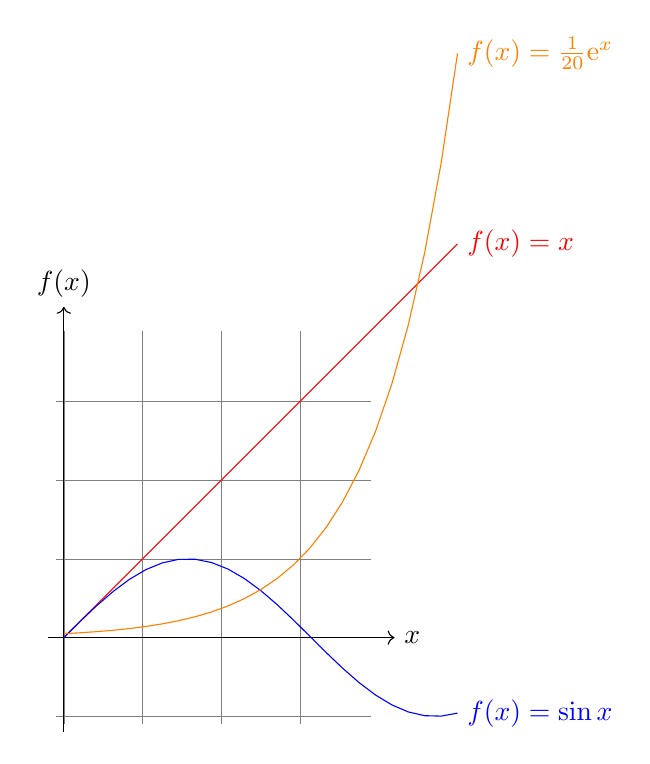
\begin{tikzpicture}[domain=0:5]
  \draw[very thin,color=gray] (-0.1,-1.1) grid (3.9,3.9);
  \draw[->] (-0.2,0) -- (4.2,0) node[right] {$x$};
  \draw[->] (0,-1.2) -- (0,4.2) node[above] {$f(x)$};
  \draw[color=red] plot (\x,\x) node[right] {$f(x) =x$};
  % \x r means to convert '\x' from degrees to _r_adians:
  \draw[color=blue] plot (\x,{sin(\x r)}) node[right] {$f(x) = \sin x$};
  \draw[color=orange] plot (\x,{0.05*exp(\x)}) node[right] {$f(x) = \frac{1}{20} \mathrm e^x$};
  \end{tikzpicture}

  \vspace{2cm}
  A two perpendicular lines
  \begin{tikzpicture}[scale =2, radius=1cm,delta angle=30]
    \draw (-1,0) -- +(3.5,0);
    \draw (1,0) ++(210:2cm) -- +(30:4cm);
    \draw (1,0) +(0:1cm) arc [start angle=0];
    \draw (1,0) +(180:1cm) arc [start angle=180];
    \path (1,0) ++(15:.75cm) node{$\alpha$};
    \path (1,0) ++(15:-.75cm) node{$\beta$};
    \end{tikzpicture}

A sample histogram graph
    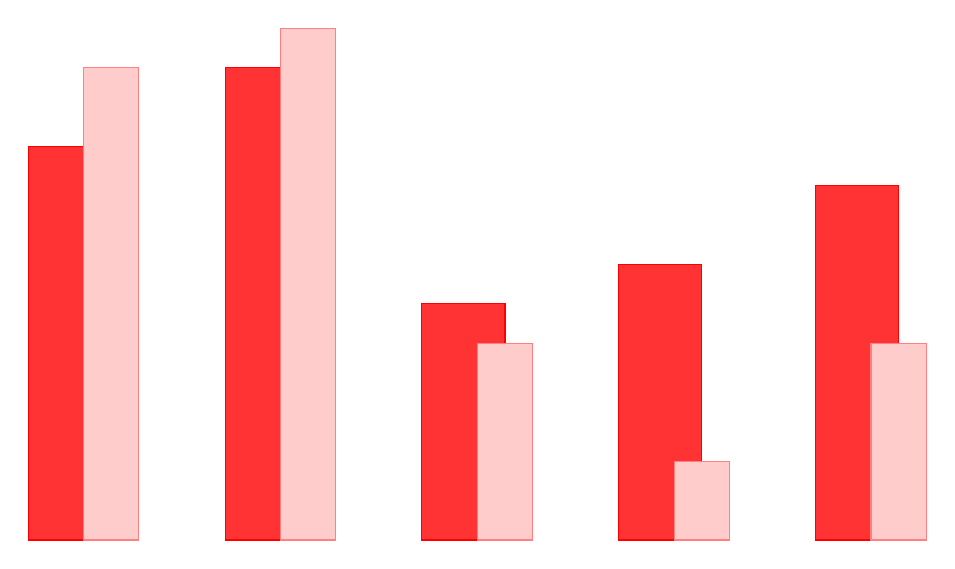
\begin{tikzpicture}[ybar, scale= 5]
      \draw[color=red,fill=red!80,bar width=6pt]
      plot coordinates{(0,1) (.5,1.2) (1,.6) (1.5,.7) (2,.9)};
      \draw[color=red!50,fill=red!20,bar width=4pt,bar shift=3pt]
      plot coordinates{(0,1.2) (.5,1.3) (1,.5) (1.5,.2) (2,.5)};
      \end{tikzpicture}
    
    
    \vspace{3cm} 
    A polynomial lines crossing each other
    \begin{tikzpicture}[xscale=3]
      \draw (0,0) sin (1,1) cos (2,0) sin (3,-1) cos (4,0) sin (5,1);
      \draw[color=red] (0,1.5) cos (1,0) sin (2,-1.5) cos (3,0) sin (4,1.5) cos (5,0);
      \end{tikzpicture}

\vspace{2cm}
data visualization in A.I
      \usetikzlibrary {datavisualization.formats.functions}
      \tikz \datavisualization
      [scientific axes,
      visualize as smooth line,
      all axes= {grid, unit length=1.25cm},
      y axis={ ticks=few },
      x axis={ ticks=many, ticks and grid={ major also at={(pi/2) as $\frac{\pi}{2}$}}}]
      data [format=function] {
      var x : interval [-pi/2:3*pi] samples 50;
      func y = sin(\value x r);
      };
      
    
% .. REFERENCES  STARTS HERE ....%
\addcontentsline{toc}{section}{\MakeUppercase{\textbf{references}}}
\bibliography{myrefs}
\bibliographystyle{apalike}
\cite{Met78}
\cite{Wel03}
\cite{Lit96}
\cite{Tho98w}


% .. APPENDIX STARTS HERE ....%
\addcontentsline{toc}{section}{\MakeUppercase{\textbf{Appendices}}}
\chapter*{\centering \MakeUppercase{Appendices}} 
\centering\textbf{\Huge{APPENDIX A:}}


% I HOPE YOUR ENJOY THE CLASS!!!!!   THANKS. UDSM STUDENTS FOR FYP.%
\end{document}
